\documentclass{article}

\usepackage{a4wide}
\usepackage[utf8]{inputenc}
\usepackage[T1]{fontenc}
\usepackage[french]{babel}
\usepackage[babel=true]{csquotes} % guillemets français
\usepackage{graphicx}
\graphicspath{{Images/}}
\usepackage{color}
\usepackage{hyperref}
\hypersetup{colorlinks,linkcolor=,urlcolor=blue}

\usepackage{amsmath}
\usepackage{amssymb}


\title{Développement pour mobiles 2 - The Fearless Glutton}
\author{Jean-Emile PELLIER, L3 informatique}
\date{\today}

\begin{document}

\maketitle % pour écrire le titre


%% Le résumé:
\begin{abstract}
Pac-Man est un jeu vidéo qui consiste à déplacer un personnage en forme de diagramme circulaire dans un labyrinthe afin qu'il puisse manger toutes les pac-gommes qui s’y trouvent en évitant des fantômes.

Au-delà de l’apparente simplicité du gameplay, la conception d’un tel jeu peut se révéler particulièrement complexe. En particulier, la volonté du concepteur d’associer à chaque fantôme une personnalité qui lui est propre au travers de ses déplacements complique significativement l’implémentation.

Dans ce document, nous allons étudier une implémentation mobile de ce jeu dans sa version originale.
\end{abstract}


\section{Introduction}
\label{section:intro} % pour faire référence à la section ailleurs (\ref{...} voir plus bas)

\textit{Pac-Man}~\cite{Pac-Man} est un jeu vidéo créé par T\={o}ru Iwatani pour l’entreprise japonaise Namco. Il est sorti sur bornes d’arcade au Japon le 22 mai 1980 puis aux Etats-Unis le 25 octobre 1980.

Le jeu consiste à déplacer un personnage du nom de Pac-Man dans un labyrinthe afin qu'il puisse manger toutes les pac-gommes et les bonus qui s’y trouvent en évitant d’être touché par des fantômes. Le labyrinthe dispose de deux passages à ses extrémités permettant aux personnages d’atteindre l’autre côté de l’écran instantanément.

Le personnage de Pac-Man ressemble à un diagramme circulaire jaune. On peut le qualifier de glouton intrépide dans la mesure où, bien qu’il se trouve dans un labyrinthe hanté, il mange tout ce qu’il peut sans réellement se soucier des fantômes, c’est bien évidemment de là que vient le nom du projet.

Chaque fantôme dispose d’une personnalité qui lui est propre, chacun d’entre eux dispose d’un nom et se comporte différemment des autres. Selon le concepteur, il s’agit d’éviter que le jeu ne soit "assommant et insipide" par la prévisibilité qu’induirait des comportements identiques dans la poursuite de Pac-Man. Il n’y a normalement pas de hasard dans les déplacements des fantômes sauf lorsqu’ils sont effrayés et qu’ils prennent la fuite.

Le fantôme rouge se nomme Blinky, il a une stratégie assez agressive, il se contente de suivre Pac-Man, il faut donc se méfier de lui en cas de demi-tour. Le fantôme rose se nomme Pinky, il a une stratégie de surprise, il tente des embuscades en se positionnant là où se dirige Pac-Man. Le fantôme bleu se nomme Inky, il a une stratégie assez imprévisible, il essaie d’atteindre un point situé à 2 fois la distance entre Blinky et deux cases après Pac-Man dans la direction de Blinky vers Pac-Man. Le fantôme orange se nomme Clyde, il a une stratégie de repli, il se rapproche de Pac-Man mais quand il est trop près il fuit vers le bord inférieur gauche.

Le jeu fonctionne sur un système de score basé sur le nombre de pac-gommes et de bonus consommés.

On distingue deux types de pac-gommes : les pac-gommes et les super pac-gommes. Les pac-gommes rapportent 10 points tandis que les super pac-gommes rapportent 50 points et effrayent les fantômes. 

On distingue huit types de bonus : les cerises, les fraises, les oranges, les pommes, les melons, les galaxians, les cloches et les clés. Ils rapportent respectivement 100, 300, 500, 700, 1000, 2000, 3000 et 5000 points.

Le joueur obtient une vie supplémentaire s’il dépasse les 10 000 points.

Une fois que tous les éléments consommables du labyrinthe ont été consommés, le joueur passe au niveau suivant, le type de bonus susceptible d’apparaitre change alors, et toutes les pac-gommes réapparaissent.

Comment peut-on implémenter tout cela sur mobile ?

Etudions en détails une implémentation mobile de ce jeu.



\section{Description générale de l'application}
\textbf{Menu principal}
\begin{center}
  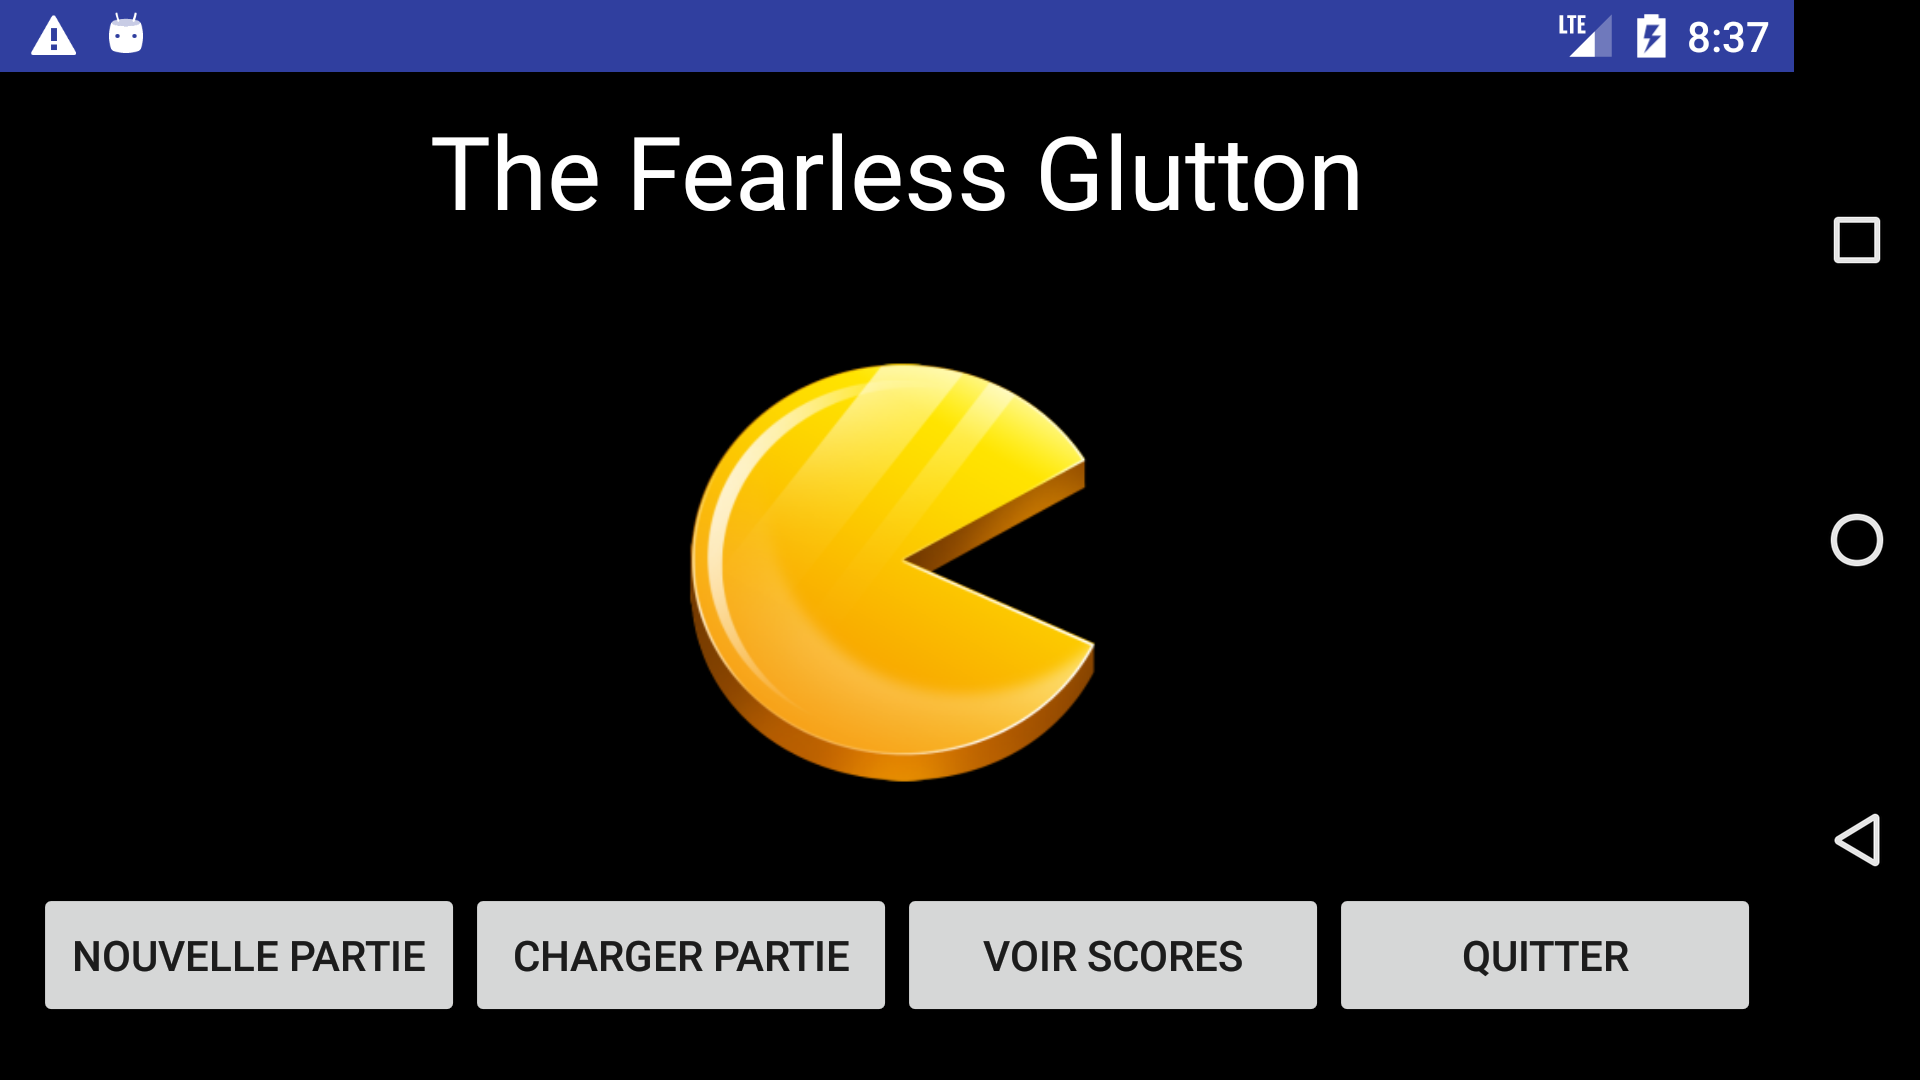
\includegraphics[scale=0.25]{MainMenuActivity.png}
\end{center}
Le menu principal offre au joueur la possibilité de :
\begin{itemize}
\item démarrer une nouvelle partie
\item charger une partie enregistrée
\item consulter les scores enregistrés
\item quitter l’application
\end{itemize}

\bigskip

\textbf{Interface de jeu}
\begin{center}
  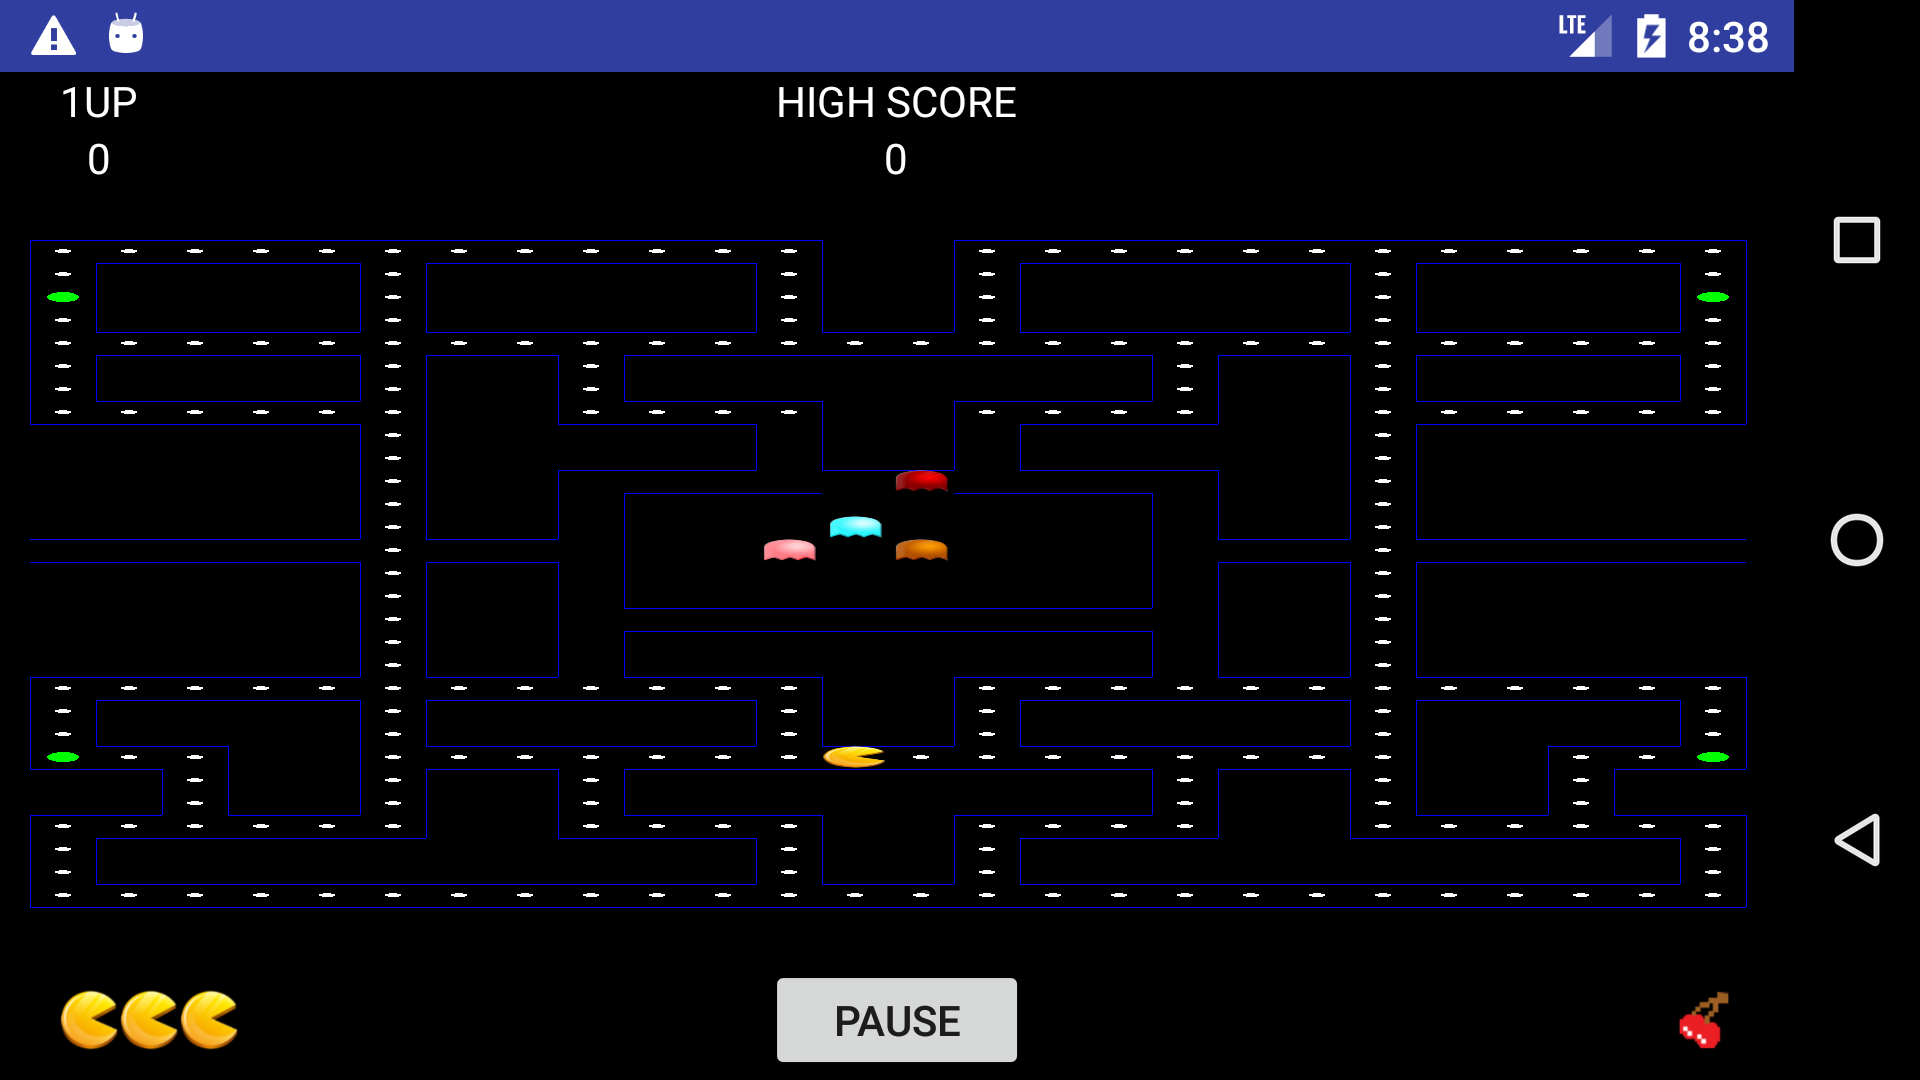
\includegraphics[scale=0.25]{GameActivity.png}
\end{center}
L'interface de jeu offre au joueur la possibilité de jouer à une version de Pac-Man très proche de la version originale.

Contrairement à la version originale, le joueur dispose de 2 fonctionnalités supplémentaires :
\begin{itemize}
\item déplacer son personnage via l'écran tactile
\item faire une pause via un bouton pause
\end{itemize}

\bigskip

\textbf{Menu pause}
\begin{center}
  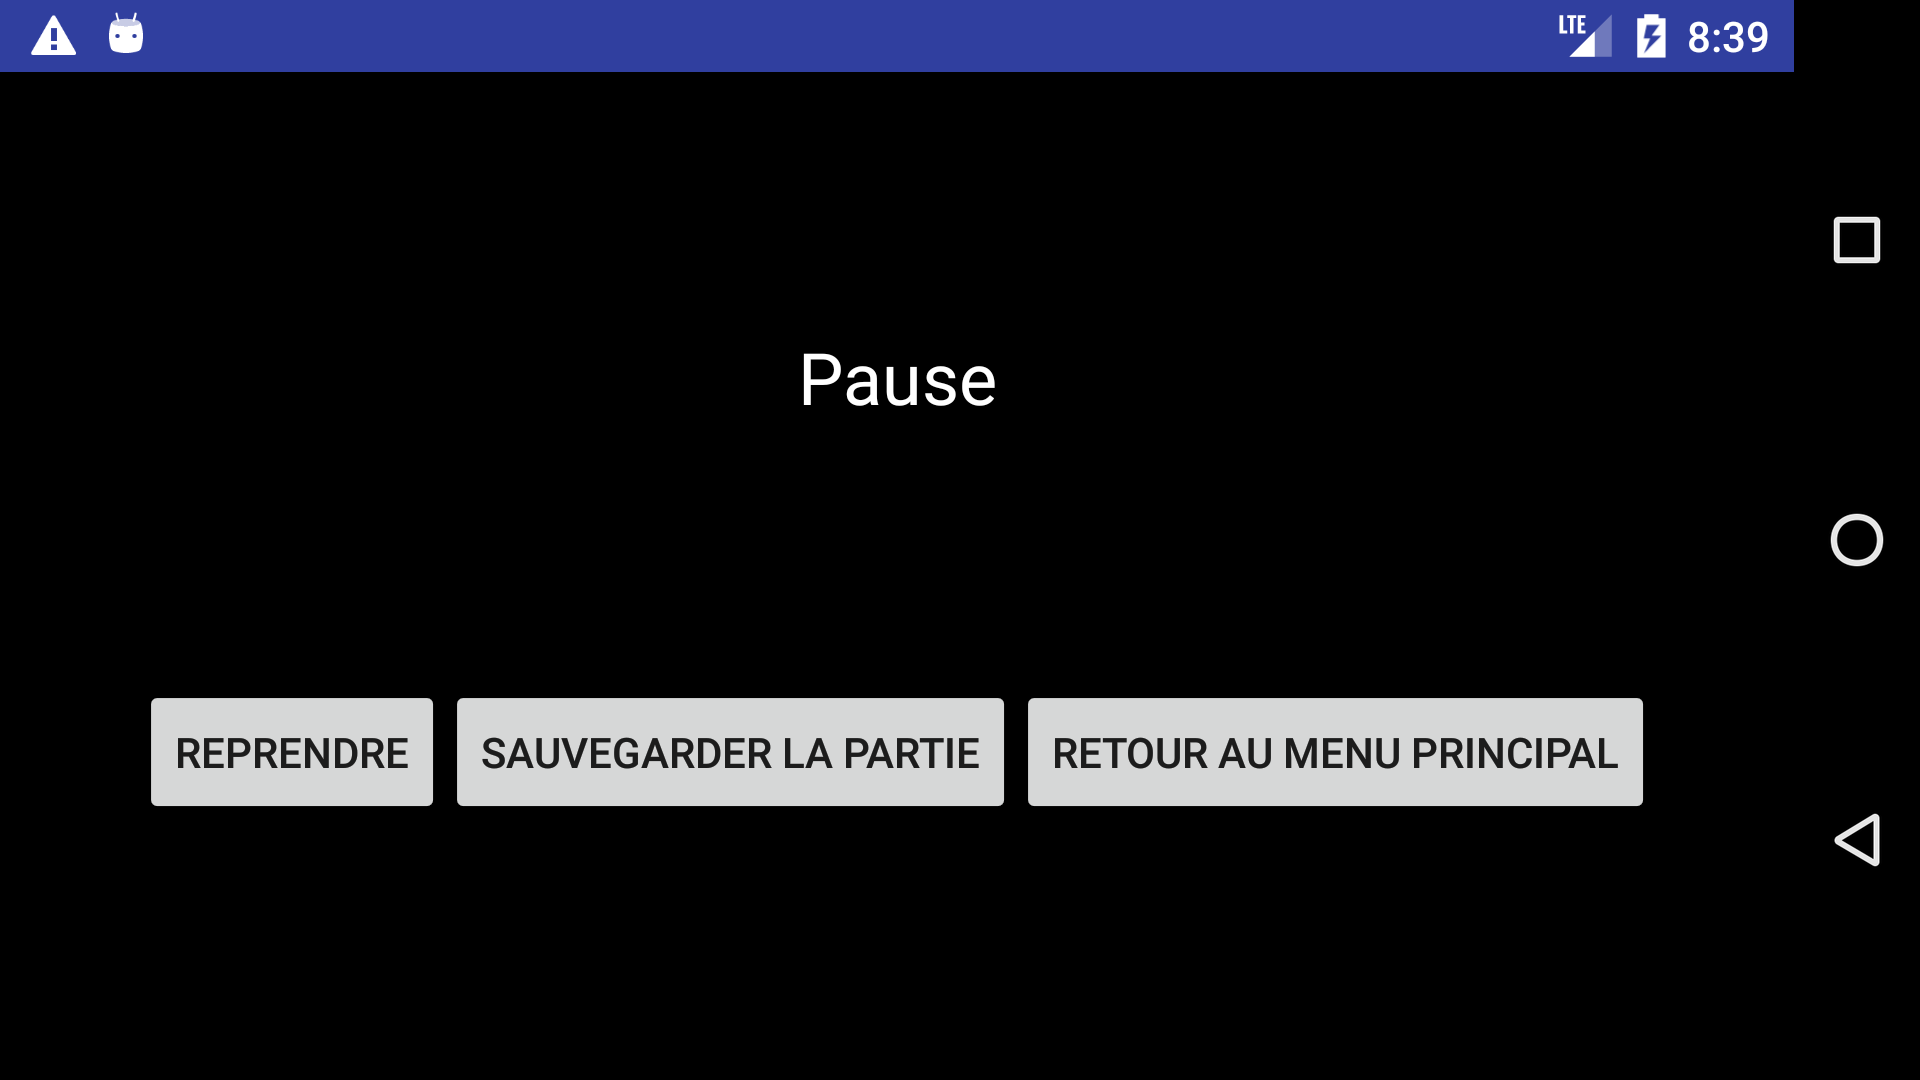
\includegraphics[scale=0.25]{PauseActivity.png}
\end{center}
Le menu pause propose au joueur de :
\begin{itemize}
\item reprendre sa partie
\item sauvegarder l’état actuel de la partie
\item retourner au menu principal
\end{itemize}

\bigskip

\textbf{Menu sauvegarder}
\begin{center}
  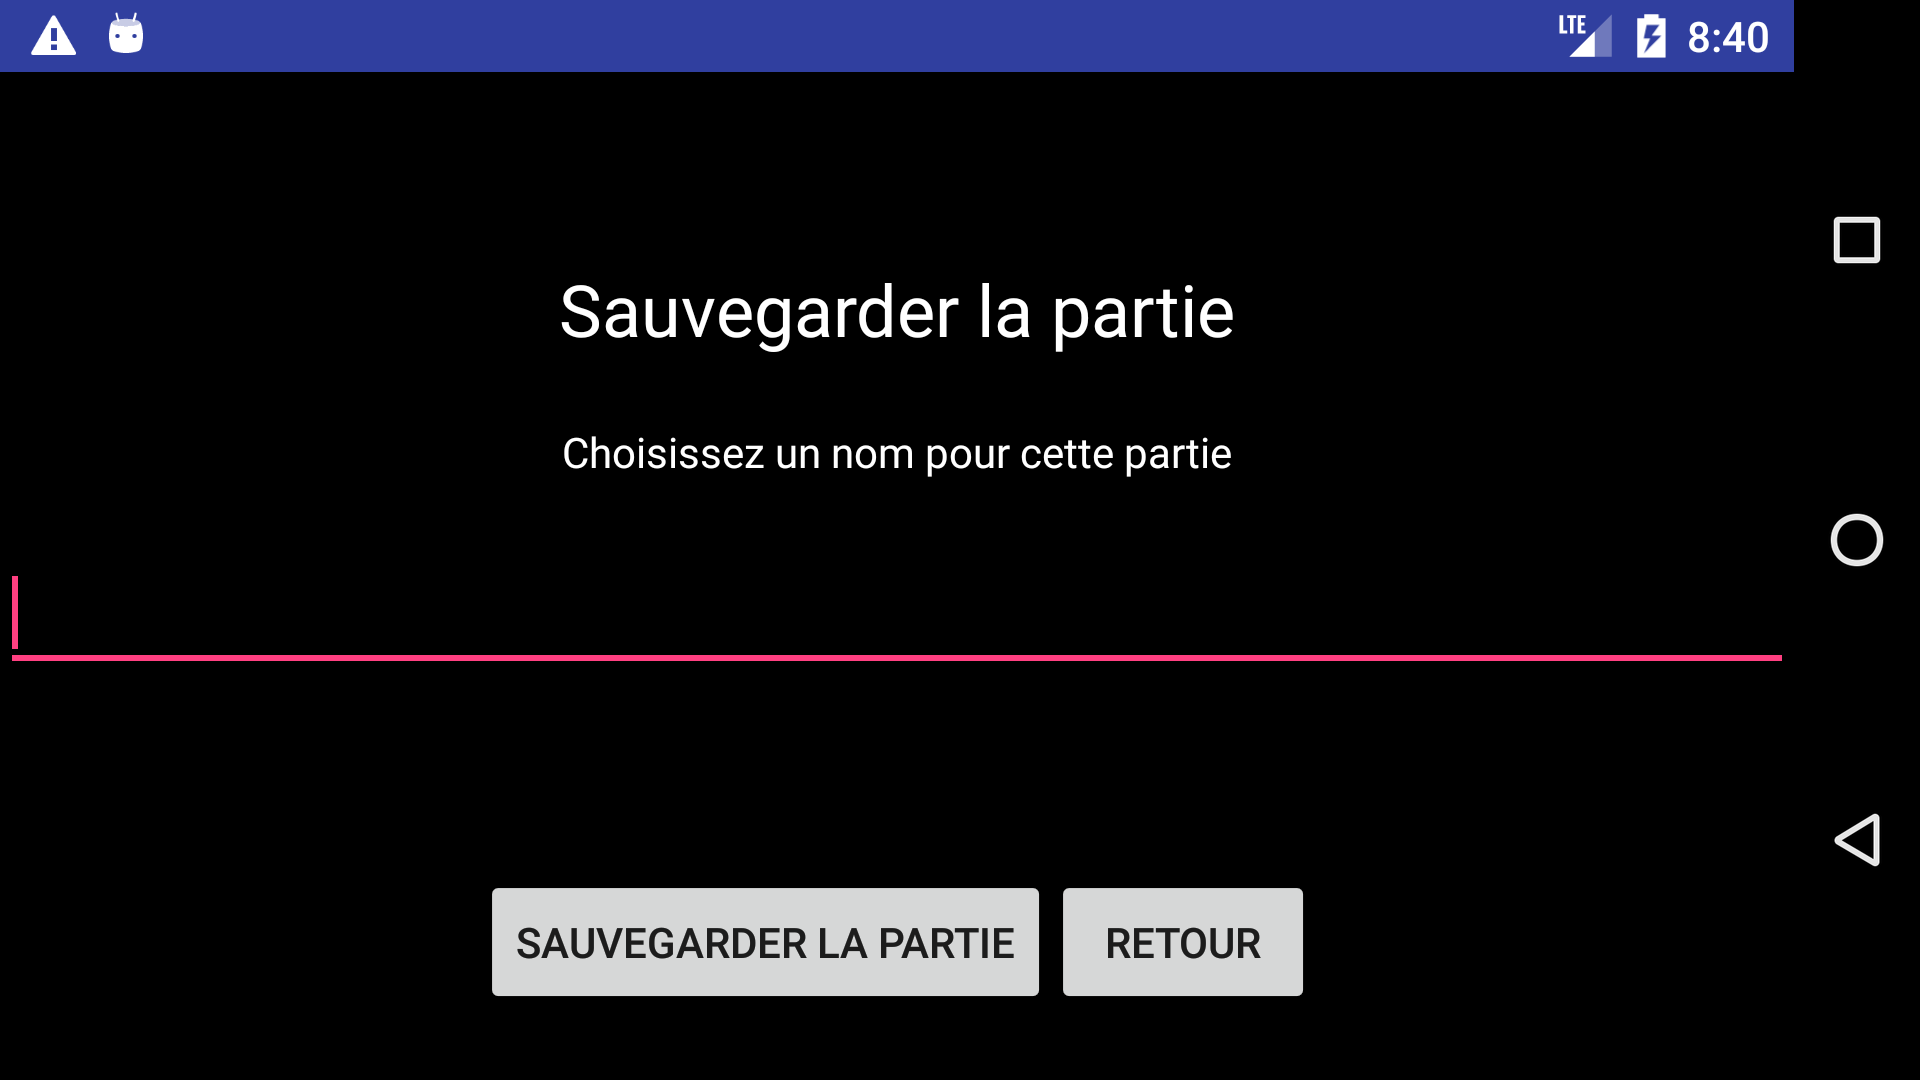
\includegraphics[scale=0.25]{SaveActivity.png}
\end{center}
Le menu de sauvegarde propose :
\begin{itemize}
\item la sauvegarde de la partie en cours
\item le nommage la partie en cours
\item le retour au menu pause
\end{itemize}

\bigskip

\textbf{Menu fin de partie}
\begin{center}
  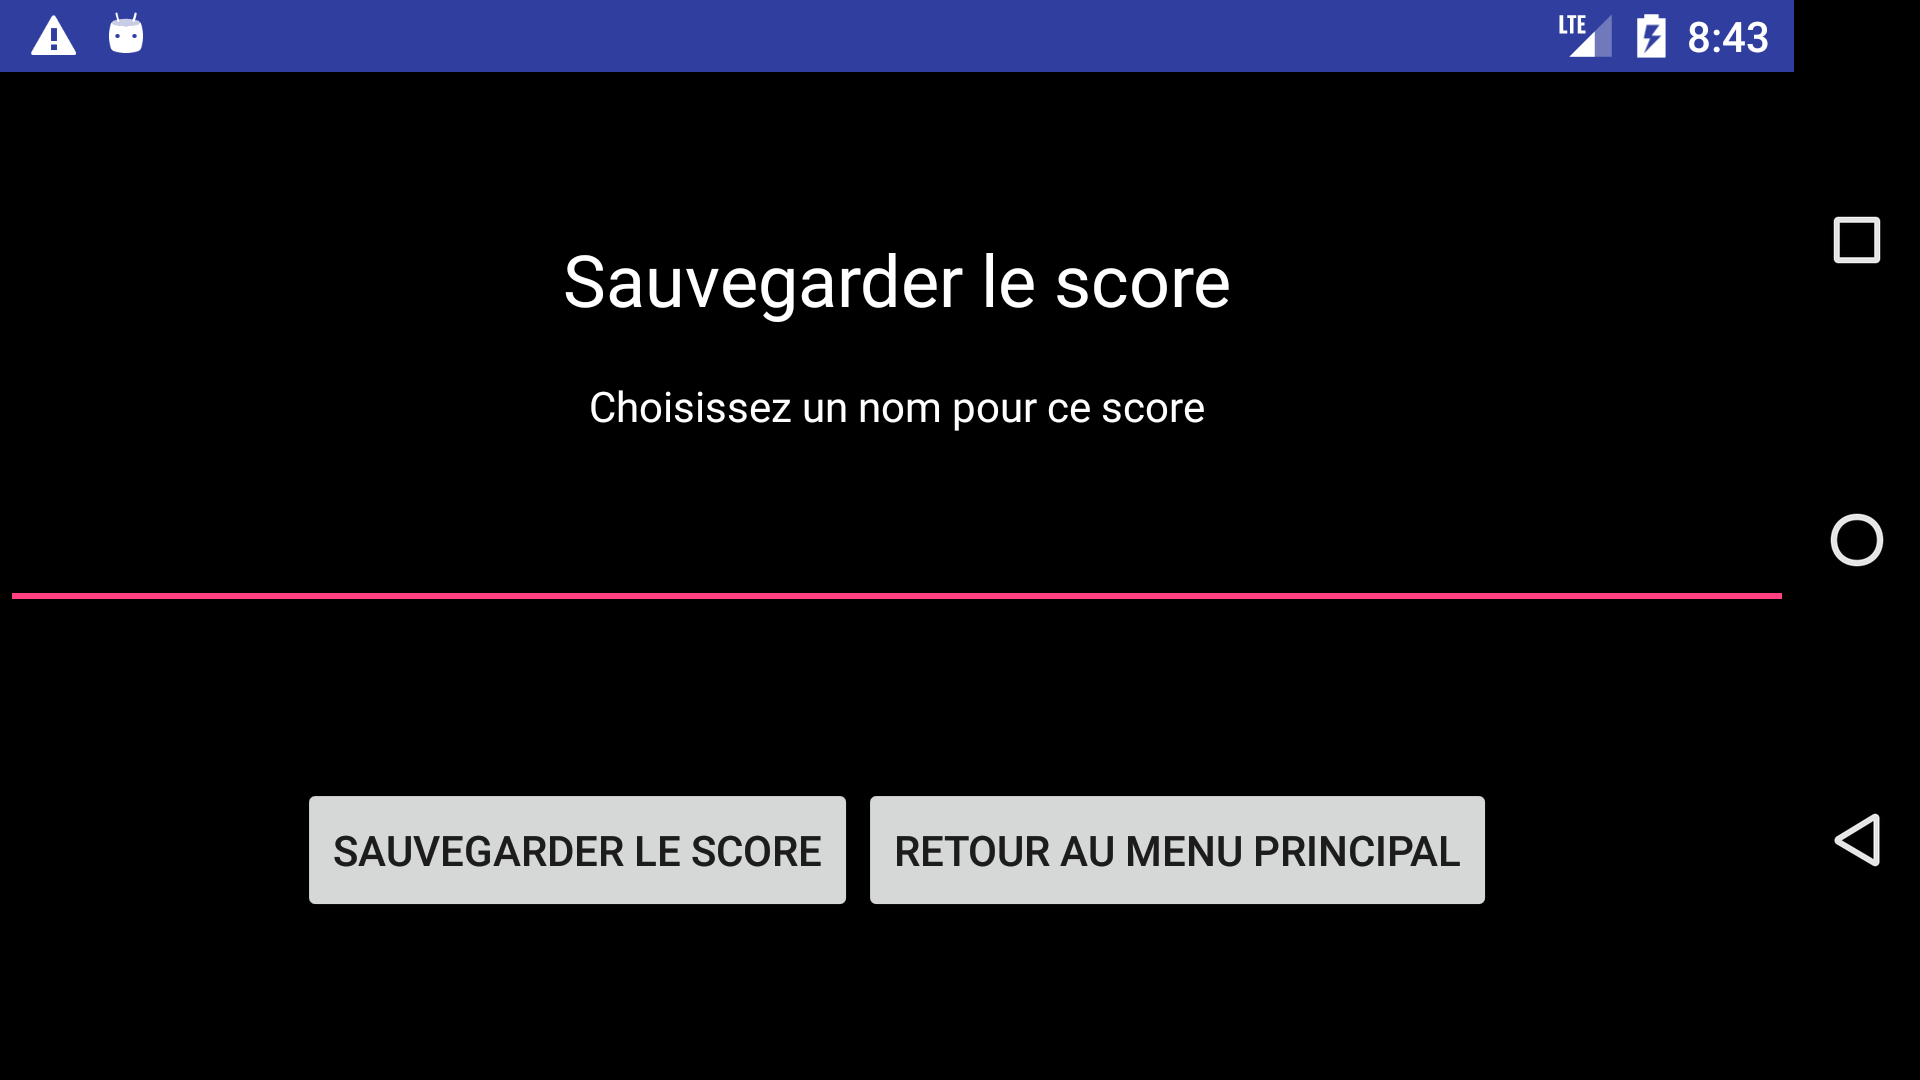
\includegraphics[scale=0.25]{GameOverActivity.png}
\end{center}
Le menu de fin de partie propose :
\begin{itemize}
\item la sauvegarde du score du joueur
\item le nommage du score
\item le retour au menu principal
\end{itemize}

\bigskip

\textbf{Menu chargement des sauvegardes}
\begin{center}
  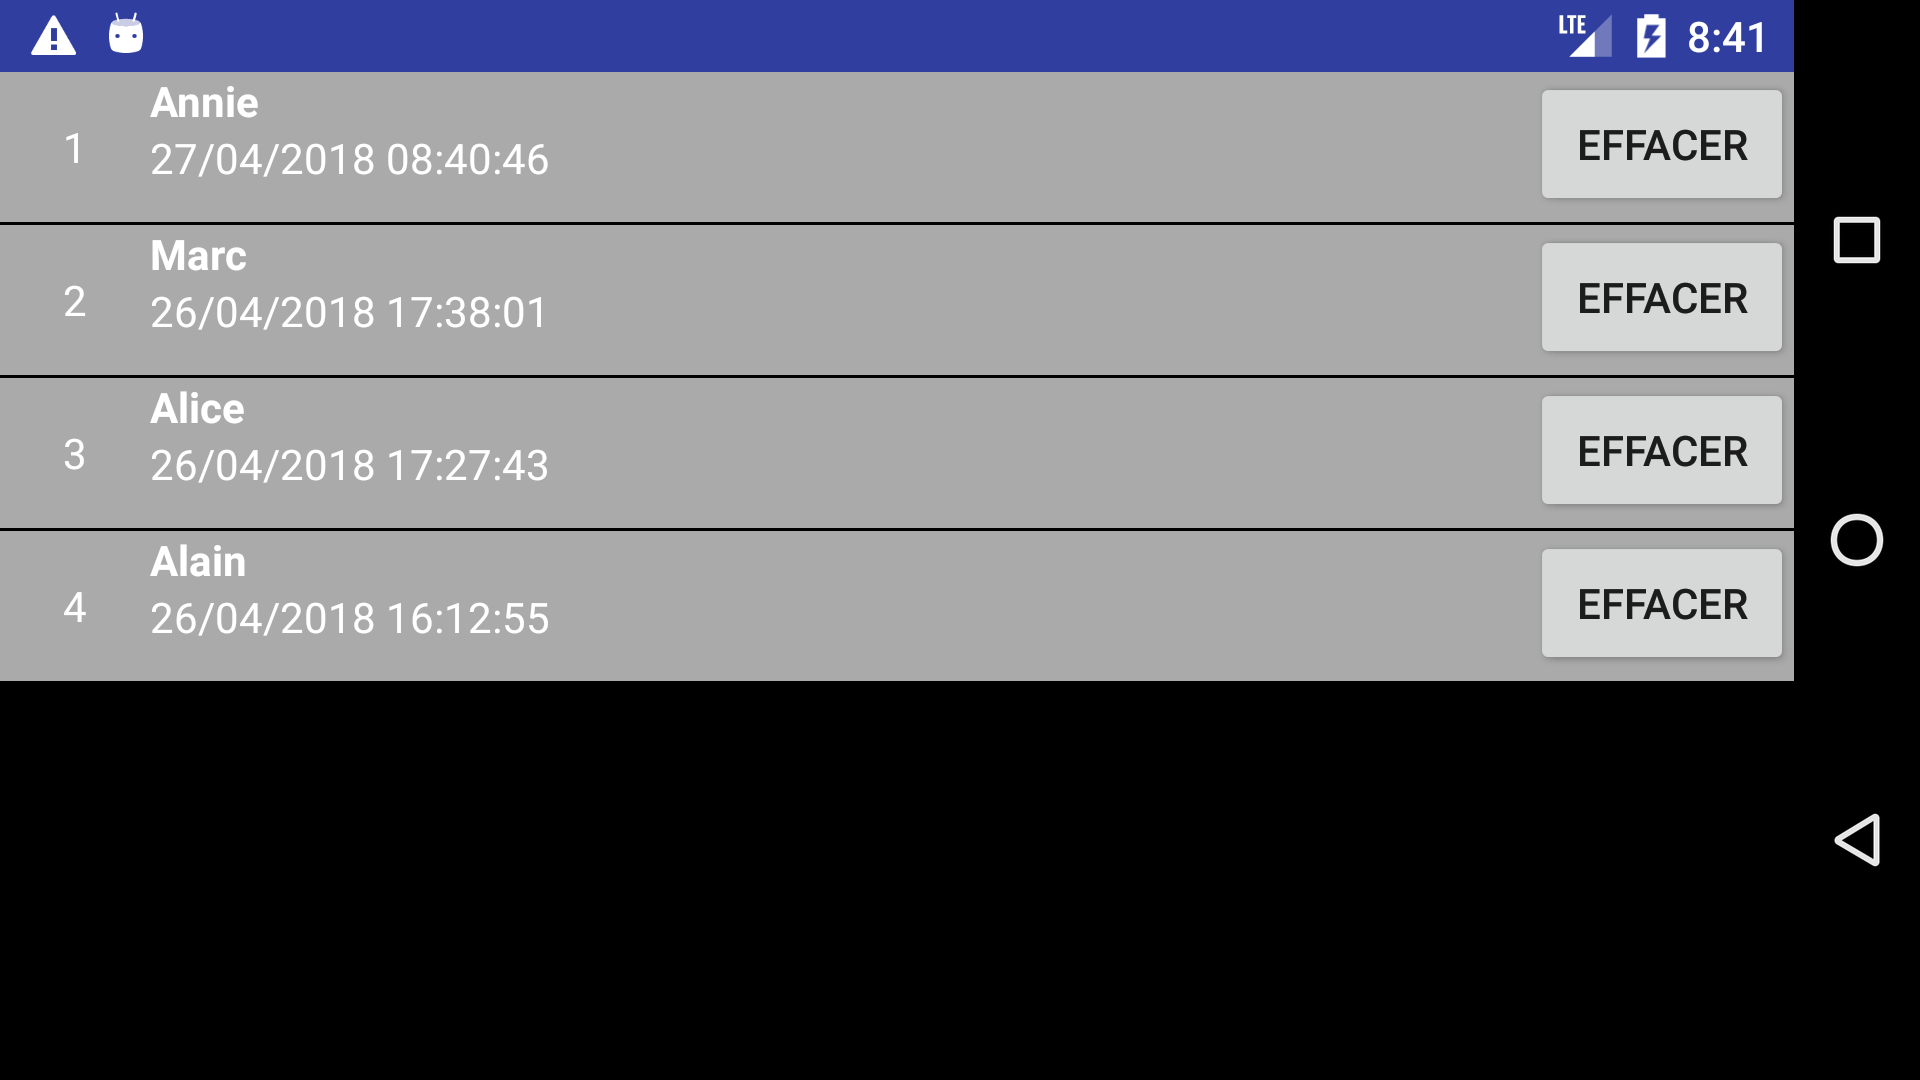
\includegraphics[scale=0.25]{LoadSaveActivity.png}
\end{center}
Le menu de chargement des sauvegardes propose :
\begin{itemize}
\item le chargement d'une partie sauvegardée
\item la consultation des parties sauvegardées
\item l'effacement d'une partie sauvegardée via le bouton effacer à droite de l'écran
\end{itemize}
Les sauvegardes sont présentées dans une liste classée par ordre chronologique décroissant.

\bigskip

\textbf{Menu affichage des scores}
\begin{center}
  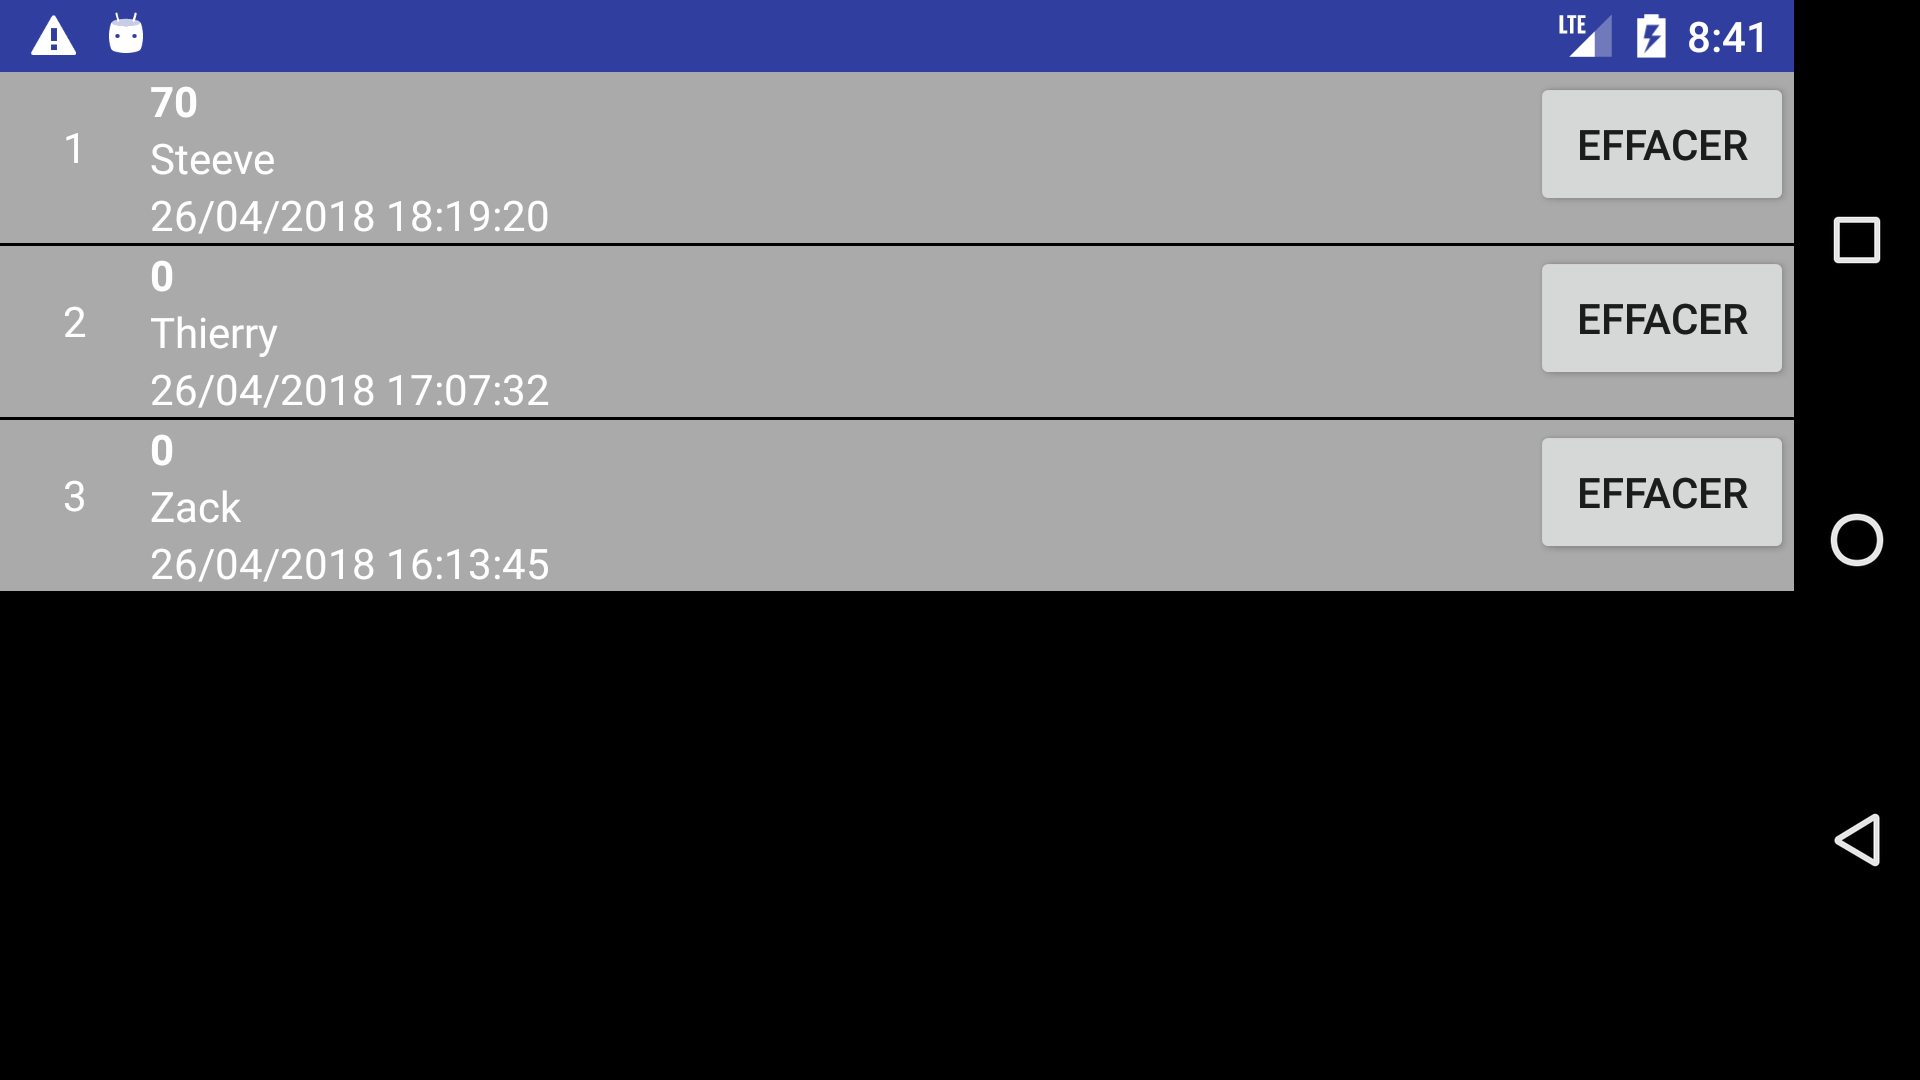
\includegraphics[scale=0.25]{ShowScoresActivity.png}
\end{center}
Le menu d’affichage des scores propose :
\begin{itemize}
\item l’affichage des scores
\item l'effacement d'un score
\end{itemize}
Les scores sont présentés dans une liste classée d’abord par ordre décroissant des scores puis par ordre alphabétique sur les noms associés aux scores.



\section{Architecture du code}
% \ref{...} permet de faire référence à un élément défini
% ailleurs dans le document (voir \label{...} plus haut).


\subsection{Android} %% une sous-section

\subsubsection{Diagramme de classe}
\begin{center}
  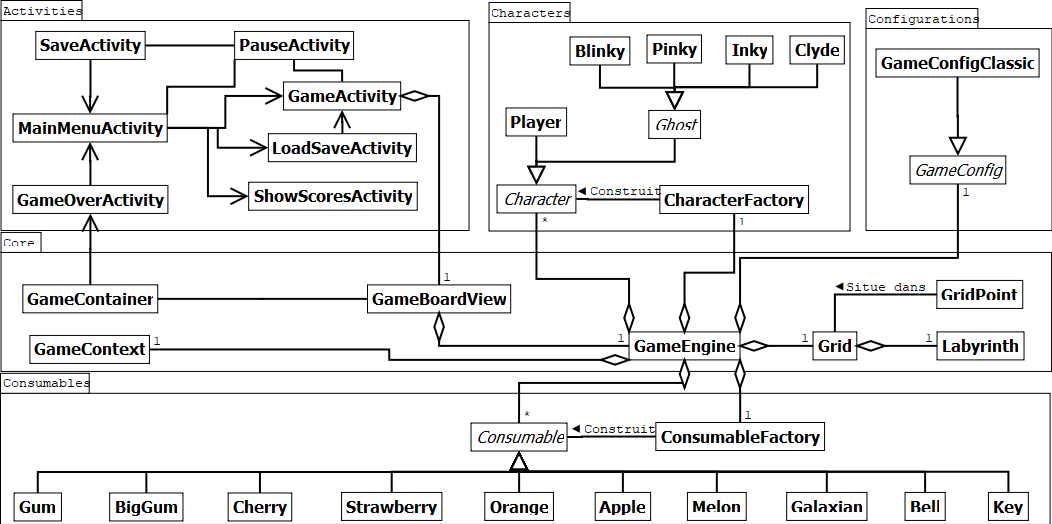
\includegraphics[scale=0.40]{ClassDiagram.png}
\end{center}
Le diagramme de classe met en évidence 5 packages que nous allons détailler.

\subsubsection{Les activités}

\medskip

\textit{MainMenuActivity}

Il s’agit de l’activité qui gère le menu principal. Elle est constituée de boutons qui permettent :
\begin{itemize}
\item de démarrer une nouvelle partie (via GameActivity avec le paramètre newGame)
\item de charger une partie existante (via LoadSaveActivity)
\item de consulter la liste des scores (via ShowScoresActivity)
\item de mettre fin à l’application
\end{itemize}

\medskip

\textit{GameActivity}

Il s’agit de l’activité qui gère le jeu. Elle est constituée :
\begin{itemize}
\item d’un plateau de jeu
\item d’une interface informant le joueur de l’état de la partie (nombres de vies, score, niveau)
\item d’un bouton pause
\end{itemize}
Le démarrage et l’arrêt du moteur de jeu s’effectuent au rythme du démarrage et de l’arrêt de cette activité. Cette activité peut démarrer avec un paramètre nickname correspondant au nom associé à une partie.
Le bouton pause va lancer l'activité PauseActivity, le 
paramètre nickname lui sera transmis.

\medskip

\textit{PauseActivity}

Il s’agit de l’activité qui gère le menu pause. Elle est constituée de boutons permettant :
\begin{itemize}
\item de reprendre la partie qui a été interrompue (via GameActivity avec le paramètre nickname)
\item de sauvegarder la partie (via SaveActivity avec le paramètre nickname)
\item de retourner au menu principal (via MainMenuActivity)
\end{itemize}

\medskip

\textit{SaveActivity}

Il s’agit de l’activité qui gère la sauvegarde de parties. Elle est constituée de boutons permettant :
\begin{itemize}
\item de sauvegarder l’état courant de la partie
\item de retourner au menu pause (via PauseActivity avec le paramètre nickname)
\end{itemize}
Un champ d'édition de texte permet de saisir un nom pour la partie.

\medskip

\textit{GameOverActivity}

Il s’agit de l’activité qui gère la fin d’une partie. Elle propose de sauvegarder le score. Elle est constituée de boutons permettant :
\begin{itemize}
\item de sauvegarder le score
\item de retourner au menu principal (via MainMenuActivity)
\end{itemize}
Un champ d'édition de texte permet de saisir un nom pour le score.

\medskip

\textit{LoadSaveActivity}

Il s’agit de l’activité qui gère le chargement des sauvegardes. Elle est constituée d'un liste ordonnée de sauvegardes. Elle permet de consulter les informations concernant les sauvegardes (les noms et les dates). Elle permet également la suppression de sauvegardes.

\medskip

\textit{ShowScoresActivity}

Il s’agit de l’activité qui gère l’affichage des scores. Elle est constituée d'un liste ordonnée de scores. Elle permet de consulter les informations concernant les scores (les scores, les noms et les dates). Elle permet également la suppression de scores.

\subsubsection{Les personnages}

\textit{Character}

Un personnage est une entité définie par son état mort ou vivant, son apparence, sa position initiale, sa position courante et le chemin qu’il est en train de suivre. Il peut mourir, ressusciter, se déplacer, entrer en collision avec un autre personnage.

\medskip

\textit{Player}

Un joueur est un personnage muni d’un certain nombre de vies. Il peut manger des consommables.

\medskip

\textit{Ghost}

Un fantôme est un personnage muni d’un état de peur, et d’une apparence spécifique s’il a peur. Le chemin que suit un fantôme est déterminé par celui d’un ou plusieurs autres personnages.

\medskip

\textit{Blinky}

Blinky est un fantôme qui a la particularité de suivre Pac-Man où qu’il aille.

\medskip

\textit{Pinky}

Pinky est un fantôme qui se positionne en embuscade.

\medskip

\textit{Inky}

Inky est un fantôme qui se positionne à deux fois la distance entre Blinky et deux cases après Pac-Man dans la direction de Blinky vers Pac-Man.

\medskip

\textit{Clyde}

Clyde est un fantôme qui suit Pac-Man mais qui fuit vers le bord inférieur gauche quand il est trop près.

\medskip

\textit{CharacterFactory}

La fabrique de personnages construit les personnages en leur attribuant une apparence et leurs positions respectives.

\subsubsection{Les consommables}

\textit{Consumable}

Un consommable modèle, définie par une classe abstraite, pour l’ensemble des consommables. Caractérisé par une position, une apparence, une catégorie et une valeur.

\medskip

\textit{Gum}

Une pac-gomme est un consommable instanciable d'une valeur de 10 points.

\medskip

\textit{BigGum}

Une super pac-gomme est un consommable instanciable d'une valeur de 50 points.

\medskip

\textit{Cherry}

Une cerise est un consommable instanciable d'une valeur de 100 points.

\medskip

\textit{Strawberry}

Une fraise est un consommable instanciable d'une valeur de 300 points.

\medskip

\textit{Orange}

Une orange est un consommable instanciable d'une valeur de 500 points.

\medskip

\textit{Apple}

Une pomme est un consommable instanciable d'une valeur de 700 points.

\medskip

\textit{Melon}

Un melon est un consommable instanciable d'une valeur de 1000 points.

\medskip

\textit{Galaxian}

Un galaxian est un consommable instanciable d'une valeur de 2000 points.

\medskip

\textit{Bell}

Une cloche est un consommable instanciable d'une valeur de 3000 points.

\medskip

\textit{Key}

Une clé est un consommable instanciable d'une valeur de 5000 points.

\medskip

\textit{ConsumableFactory}

La fabrique de consommables construit les consommables. Elle distingue les pac-gommes et les bonus. Les pac-gommes définissent elles-même leur apparence et apparaissent à des emplacements précis définis par le paramétrage de jeu tandis que les bonus nécessitent des images pour leur apparence et apparaissent à des emplacements choisis par la fabrique.

\subsubsection{Les configurations}

\textit{GameConfig}

Le paramétrage de jeu définit un modèle de paramètres à fournir au jeu pour un fonctionnement cohérent.

\medskip

\textit{GameConfigClassic}

Le paramétrage de la version originale définit des paramètres pour que le jeu ressemble à la version originale.

\subsubsection{Le cœur}

\textit{GameBoardView}

La vue du plateau de jeu définit la vue avec laquelle l'utilisateur peut intéragir dans le cadre du jeu.

\medskip

\textit{GameContainer}

Le conteneur de jeu étend la portée du moteur de jeu à l'ensemble des vues de l'activité GameActivity.

\medskip

\textit{GameContext}

Le contexte de jeu est une structure regroupant les données que l’on peut sauvegarder.

\medskip

\textit{GameEngine}

Le moteur de jeu gère l'intégralité des mécanismes de jeu. Il utilise un thread temporisé pour traiter le cycle des évènements de jeu.
Les personnages et les consommables sont protégés contre les accès concurrents car ils participent au cycle des évènements de jeu et sont dessinés par des threads distincts.

\medskip

\textit{Grid}

La grille définit l’univers bidimensionnel du jeu. Aucun élément du jeu ne peut se trouver en dehors de cette grille. La recherche des chemins des différents personnages s'effectue à partir de cette grille.

\medskip

\textit{GridPoint}

Un point de grille est une position dans la grille. Il contient les méthodes hashCode et equals pour l'utilisation des collections manipulant le hachage.

\medskip

\textit{Labyrinth}

Le labyrinthe est une entité constituée de parois qu'il positionne en fonction du paramétrage de jeu. 


\subsection{iOS} %% une autre sous-section
Implémentation abandonnée

\section{Quelques points délicats/intéressants}

\subsection{L’algorithme de Dijkstra}

L'\textit{algorithme de Dijksta}~\cite{algoDijkstra} n'est pas en soi une difficulté mais, étant donné son importance dans la détermination des chemins des personnages, il faut veiller à l'implémenter correctement. En particulier, l'algorithme ne termine pas si on lui demande un chemin entre deux points alors qu'il n'en existe pas, la solution adoptée pour ce problème dans le projet est de renvoyer un chemin vide. De plus, bien que l'algorithme fonctionne bien même en présence de graphes disjoints, on peut préalablement identifier l'unique graphe accessible par le joueur pour accélérer le traitement de l'algorithme.

\subsection{SharedPreferences}

Les \textit{SharedPreferences}~\cite{sharedPreferences} servent à sauvegarder certains objets pour une utilisation ultérieure. Toutefois, certains objets ne peuvent être sauvegardés tels quels, il va falloir créer une représentation textuelle de l'objet.

\subsection{Les collections}

Les \textit{collections}~\cite{collections} sont des objets permettant de gérer des ensemble d'objets. Elles permettent notamment de simplifier certains traitements comme l'identification de doublons ou encore le triage d'éléments.
Dans le cadre du projet, on utilise HashMap pour indicer les personnages par leurs noms et ainsi profiter du polymorphisme par itération sur ses éléments.
On se sert également de TreeSet pour ordonner les listes de sauvegardes et de scores.

\subsection{La concurrence}

La \textit{concurrence}~\cite{concurrence} est un problème à ne surtout pas négliger, des dysfonctionnements majeurs inopinés peuvent survenir simplement parcequ'on ne s'est pas rendu compte que le thread de dessin utilise les attributs d'un objet.

Dans le cadre du projet, les collections permettent de protéger certains accès concurrents. Toutefois, il ne s'agit pas d'une solution miracle. On notera l'utilisation d'une méthode waitInflate dans le projet qui force la synchronisation en permettant d'attendre la construction des vues afin d'éviter une modification sur une vue non construite.

\subsection{La gestion de la mémoire}

Bien que les appareils Android semblent être capables de traiter de grands ensembles de données, il est préférable de surveiller l’utilisation la mémoire. En effet, en cherchant l’équivalent concurrent pour le type ArrayList on tombe un peu trop souvent sur CopyOnWriteArrayList.
Or, cette implémentation imposant la duplication de la liste à chaque écriture n’est pas forcément souhaitable. Pour le stockage de la liste des pac-gommes, elle ne convient clairement pas puisque la liste contient un peu plus de 300 éléments et les opérations sur celles-ci ne sont que la décrémentation du nombre d'éléments lorsque pac-man les mangent.

Le labyrinthe n'est pas recontruit à chaque cycle de dessin, il est construit puis mémorisé dans une bitmap pour les cycles suivants.

\subsection{L’architecture du code}

L’étape de conception est particulièrement lourde dans ce projet, le diagramme de classe peut permettre de faciliter l’implémentation. C'est sans doute le meilleur moyen de s'apercevoir qu'une méthode ou un attribut est mal placé ou encore un moyen de construire des signatures pertinentes comme celle qui suit, issue de la classe Ghost.
\begin{verbatim}
  public abstract void updatePath(Grid, ConcurrentHashMap<String, Character>);
\end{verbatim}

\section{Conclusion}

Un jeu comme Pac-Man est particulièrement intéressant à étudier car, bien qu’il s’agisse d’un jeu relativement simple en comparaison avec ce qui se fait de nos jours, il se prête facilement à l’utilisation d’outils avancés tels que les collections, la concurrence, les fabriques, l’héritage ou encore le polymorphisme.

L’implémentation mobile dont il est question dans ce document a été pensée pour être aussi fidèle que possible à la version originale. Il avait été prévu initialement une implémentation complète du jeu mais, par manque de temps, il a fallu renoncer à certaines corrections de bugs, à diverses optimisations et même à certaines clarifications du code.

Cette implémentation prévoit l’évolution future du code notamment par l’ajout de nouveaux paramètres de jeux.

Des dysfonctionnements subsistent évidemment, une lourde phase de test pourrait bien être nécessaire avant d'obtenir une version vraiment opérationnelle.


%%% La bibliographie:
\bibliographystyle{plain}
\bibliography{biblio}

\end{document}
